\chapter{Resultados}
\label{cap:implementacaoresultados}

Neste capítulo será apresentada a metodologia de testes utilizada para validar o ambiente de alta disponibilidade criado. Após a execução
dos testes serão apresentados os resultados obtidos.

%Neste capítulo será apresetado o projeto de implementação, detalhado a implementação com a configuração do \ac{OS}, do ambiente virtualizado e 
%das ferramentas que irão compôr o \textit{cluster} de alta disponibilidade. Posteriormente, será apresentada a metodologia de testes e 
%apresentado os resultados das medições para validação da alta disponibilidade.

\section{Testes realizados}
\label{section:testes}

A metodologia de testes deste trabalho foi fundamentada nos trabalhos de \citet{reis2009} e \citet{goncalves2009}, a mesma foi desenvolvida para 
possibilitar a análise e eficácia do ambiente de alta disponibilidade. Exemplificar e detalhar ... ??
%O objetivo desta seção é comprovar que a gerência de falhas é importante para um ambiente computacional, além de destacar que a gerência da 
%manutenção também é favorecida por esta implementação.

%Os testes desenvolvidos estão detalhados nas próximas seções, neles tem-se a justificativa, a aplicação e os resultados obtidos.
Os três testes descritos nas próximas seções foram efetuados no ambiente de alta disponibilidade com uma máquina virtual para fins de experimento, 
por possuírem risco de perda de dados em sua execução.
Todavia, na Seção \ref{section:comparacaofinal} será feita a medição e a análise do período de um mês no ambiente de alta disponibilidade,
sendo que neste ambiente estarão executando os serviços críticos definidos.

\subsection{Teste 1 - Desligamento físico}
%Desligamento físico (simulação falha de hardware ou eletrica): 4 vezes para medir tempo de downtime dos serviços e dos nodes (servico não crítico)

Este teste faz a simulação de falhas de \textit{hardware} ou falhas elétricas em um nó do \textit{cluster}. Com este teste pode-se validar ainda 
o processo de \textit{failover} dos serviços (máquinas virtuais) que estavam executando no nó que falhou, bem como medir o tempo de 
indisponibilidade dos serviços.

%O procedimento deste teste é o seguinte:
%\begin{itemize}
% \item Acessar o terminal do servidor de monitoramento;
% \item Executar comando \textit{ping} e medir o tempo de indisponibilidade (\textit{script} no Apêndice \ref{ap:scriptindisp});
% \item Forçar desligamento do nó;
% \item Aguardar máquinas virtuais inicirem no outro nó;
% \item Finalizar a medição do tempo e \textit{ping}.
%\end{itemize}

Este procedimento foi executado 4 vezes, sendo aplicado 2 vezes em cada nó. A Tabela \ref{tab:teste1resultadosvirt} possui os dados 
resultantes dos testes e das medições efetuadas sobre a máquina virtual.
% feito em 15/09

\begin{table}[h!]
\caption{Resultados do teste 1 com servidor virtual.}
\label{tab:teste1resultadosvirt}
\begin{center}
\begin{tabular}{|l|p{2.2cm}|p{2.5cm}|p{2cm}|p{2.7cm}|}\hline
 & \textbf{Pacotes transmitidos} & \textbf{Percentual de pacotes perdidos} & \textbf{Latência média} & \textbf{Tempo de indisponibilidade} \\\hline
Teste 1 & 301 & 0 & 0,21 ms & 0 segundos \\\hline
Teste 2 & 301 & 0 & 0,22 ms & 0 segundos \\\hline
Teste 3 & 189 & 37 & 7,06 ms & 86 segundos \\\hline
Teste 4 & 216 & 28 & 4,96 ms & 76 segundos \\\hline
Média & 251,75 & 16,25 & 3,11 ms & 40,5 segundos \\\hline
\end{tabular}
\end{center}
\end{table}

Pode-se observar que o tempo de indisponibilidade da máquina virtual é baixo, uma vez que é iniciada em um outro nó logo após o desligamento do 
primeiro nó. Destaca-se que o \ac{MTTR} seria significativamente maior caso fosse necessário reconfigurar a máquina virtual, reinstalar as 
aplicações, configurá-las e restaurar o \textit{backup}. Dependendo do servidor e da aplicação, a indisponibilidade poderia ser maior que 24 horas.

Na Tabela \ref{tab:teste1resultados} tem-se as médias dos testes dos servidores físicos, pode-se perceber o elevado percentual de pacotes perdidos. 
Além disso, percebe-se a diferença do tempo de indisponibilidade da máquina virtual que é de 40,5 segundos comparado com os servidores 
físicos que são de 169 e 205,5 segundos.

\begin{table}[h!]
\caption{Resultados do teste 1 dos servidores físicos.}
\label{tab:teste1resultados}
\begin{center}
\begin{tabular}{|l|p{2.2cm}|p{2.5cm}|p{2cm}|p{2.7cm}|}\hline
 & \textbf{Média dos pacotes transmitidos} & \textbf{Média do percentual de pacotes perdidos} & \textbf{Latência média} & \textbf{Média do tempo de indisponibilidade} \\\hline
Nó 1 & 300,5 & 58,5 & 20,68 ms & 169 segundos \\\hline
Nó 2 & 300,5 & 69,5 & 31,44 ms & 205,5 segundos \\\hline
\end{tabular}
\end{center}
\end{table}

A Figura \ref{fig:teste1_disponibilidade} demonstra a disponibilidade dos servidores físicos \textit{Brina} (Nó 1) e \textit{Piova} (Nó 2) e da 
máquinas virtual (\textit{Trapel}). A máquina virtual teve apenas 1 minuto e 10 segundos de \textit{downtime}, deste modo, caso o 
\textit{hardware} o qual a máquina virtual está executando falhe, o serviço será reestabelecido neste curto período de tempo.

\begin{figure}[h!]
 \centering
 \includegraphics[width=470px]{img/teste1_disponibilidade.eps}
 \caption{Disponibilidade servidores físicos \textit{Brina} e \textit{Piova} e da máquina virtual \textit{Trapel}.}
 \label{fig:teste1_disponibilidade}
\end{figure}


\subsection{Teste 2 - Manutenção agendada}
%Agendamento de manutenção (reboot para atualização de software): 2 semanas ou mais, 1 manutenção por semana, com live migration, reboot e 
%atualizacao de kernel dos nodes. Resultados: latencia, comparacao downtime servidor virtual e fisico, log

Reinicializações são necessárias para manutenções de \textit{hardware}, atualização de \textit{software} e até mesmo para rejuvenescimento de
\textit{software} \cite{melo2014}. Desta forma, criou-se esse teste para simular manutenções previamente agendadas. Para tanto, criou-se 
um \textit{script}, disponível no Apêndice \ref{ap:scriptmanutencao}, que é responsável por migrar as \acp{VM} e reiniciar o nó.

%O procedimento deste teste é o seguinte:
%\begin{itemize}
% \item Executar comando \textit{ping} e medir o tempo de indisponibilidade (\textit{script} no Apêndice \ref{ap:scriptindisp});
% \item Executar o \textit{script} que desativa o nó (comando \textit{standby}) e executa o \textit{reboot} (Apêndice \ref{ap:scriptmanutencao});
% \item Após retorno do nó executar novamente o \textit{script} anterior para retorno do nó ao \textit{cluster};
% \item Finalizar a medição do tempo e \textit{ping}.
%\end{itemize}

Este teste foi executado 2 vezes em cada nó, durante 2 semanas. Para a execução dos \textit{scripts} foi utilizada a ferramenta 
\textit{crontab} do \textit{Linux}. Com os dados obtidos criou-se a Tabela \ref{tab:teste2resultados}.
Pode-se observar que não houve \textit{downtime} e nem perda de pacotes na máquina virtual, desta forma também não houve indisponibilidade nos 
seus serviços. Já nos nós do \textit{cluster} tem-se um tempo de indisponibilidade devido a reinicialização do servidor.
% feito em 17/09 a 30/09
% crontab brina:
% */10 04 * * 2 /usr/local/sbin/script_pacemaker_manutencao.sh
% crontab piova:
% */10 04 * * 4 /usr/local/sbin/script_pacemaker_manutencao.sh
% crontab monit:
%59 03 * * 2 cd /home/bruno/pacemaker/teste2/; bash indisponibilidade.sh 186.195.16.14 1
%59 03 * * 2 cd /home/bruno/pacemaker/teste2/; bash indisponibilidade.sh 186.195.16.13 1
%59 03 * * 4 cd /home/bruno/pacemaker/teste2/; bash indisponibilidade.sh 186.195.16.6 2
%59 03 * * 4 cd /home/bruno/pacemaker/teste2/; bash indisponibilidade.sh 186.195.16.13 2


\begin{table}[h!]
\caption{Resultados do teste 2.}
\label{tab:teste2resultados}
\begin{center}
\begin{tabular}{|l|p{2.5cm}|p{2.5cm}|p{1.5cm}|p{3cm}|}\hline
\textbf{Tipo} & \textbf{Média dos pacotes transmitidos} & \textbf{Média do percentual de pacotes perdidos} & \textbf{Latência média} & \textbf{Média do tempo de indisponibilidade} \\\hline
Nó 1 & 301 & 39,5 & 22,63 ms & 145,5 segundos \\\hline
Nó 2 & 300,5 & 44,5 & 19,8 ms & 174 segundos\\\hline
Servidor virtual & 301 & 0 & 0,309 ms & 0 segundos \\\hline
\end{tabular}
\end{center}
\end{table}

%NAO Porém, tem-se uma latência maior durante o processo de \textit{live migration}, como pode ser observado na Figura X.

Como era esperado, durante o processo de \textit{live migration} a latência da máquina virtual aumentou, isso pode ser observado na Figura 
\ref{fig:teste2_latencia} através do pico ocorrido entre os valores 50 e 100.
%teste2/186.195.16.13-stat-1.log
%teste2/186.195.16.13-stat-2.log
\begin{figure}[h!]
 \centering
 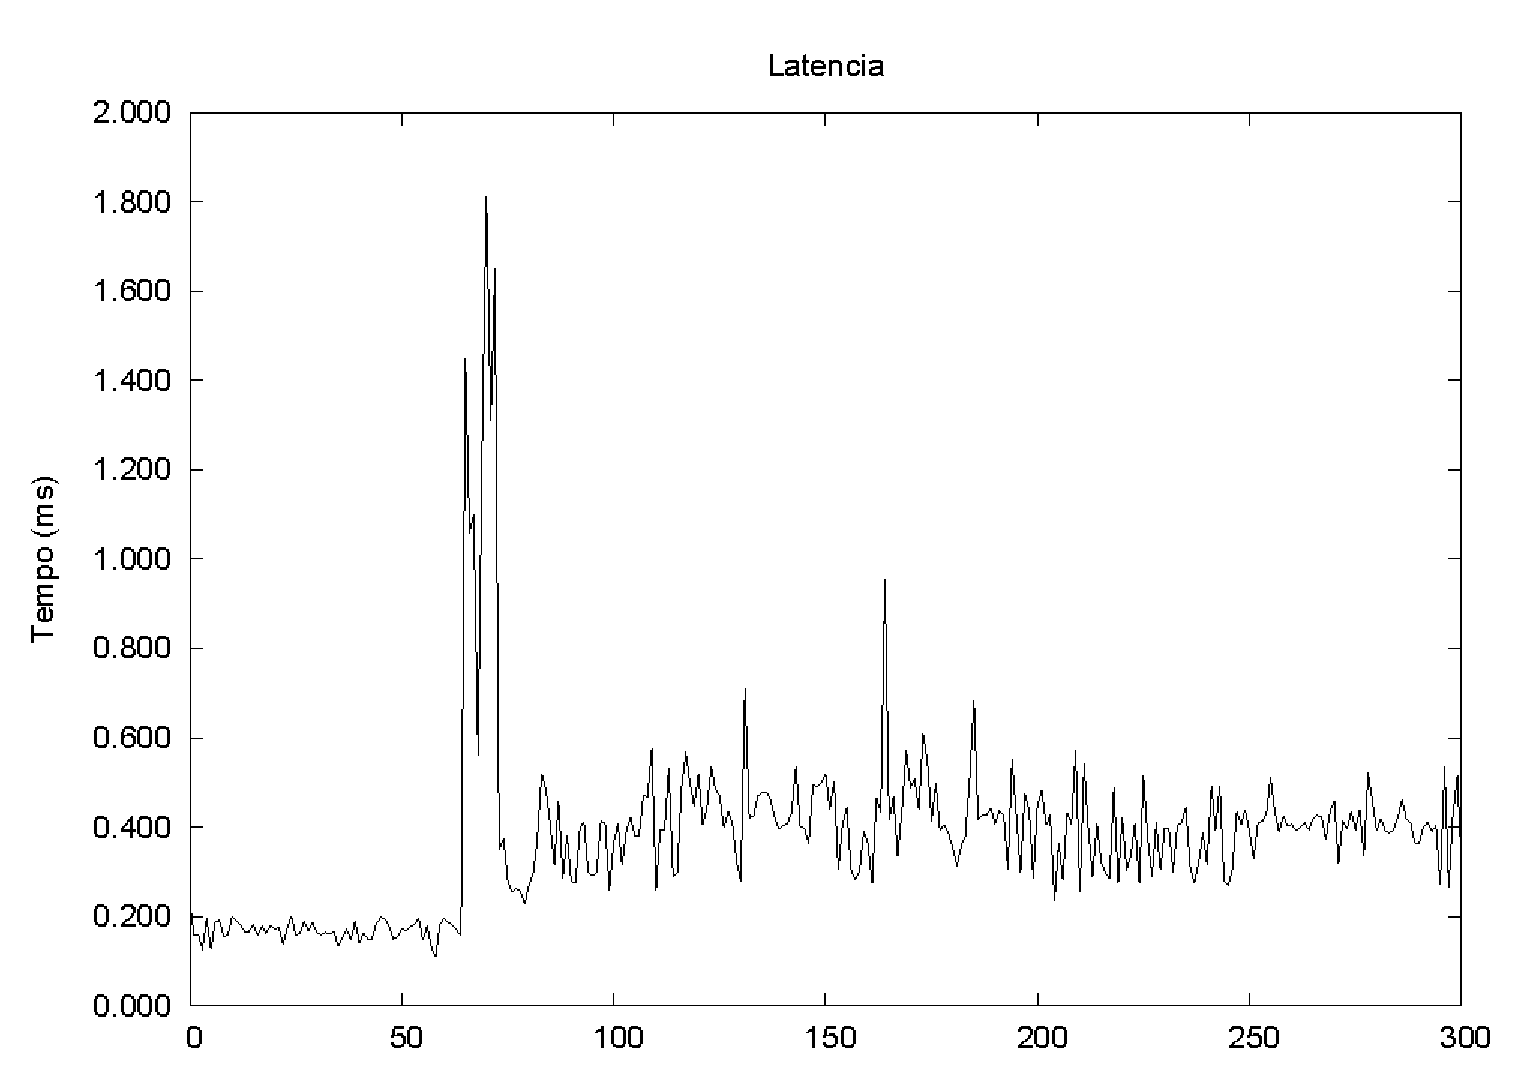
\includegraphics[width=350px]{img/teste2_latencia.eps}
 \caption{Latência da máquina virtual durante o \textit{live migration}.}
 \label{fig:teste2_latencia}
\end{figure}

A Figura \ref{fig:teste2_trapel1} demonstra a disponibilidade da máquina virtual, onde pode-se perceber que não houve nenhuma indisponibilidade. 
Esses dados foram produzidos pela ferramenta de monitoramento da empresa, \textit{Nagios}. 
%grafico comparativo nagios da disponibilidade do servidor fisico e do virtual
%grafico nagios - Trends(grafico) ou Availability (resumo) - Hosts - servidor - tempo 18/09 a 30/09 + Include Soft States = yes
\begin{figure}[h!]
 \centering
 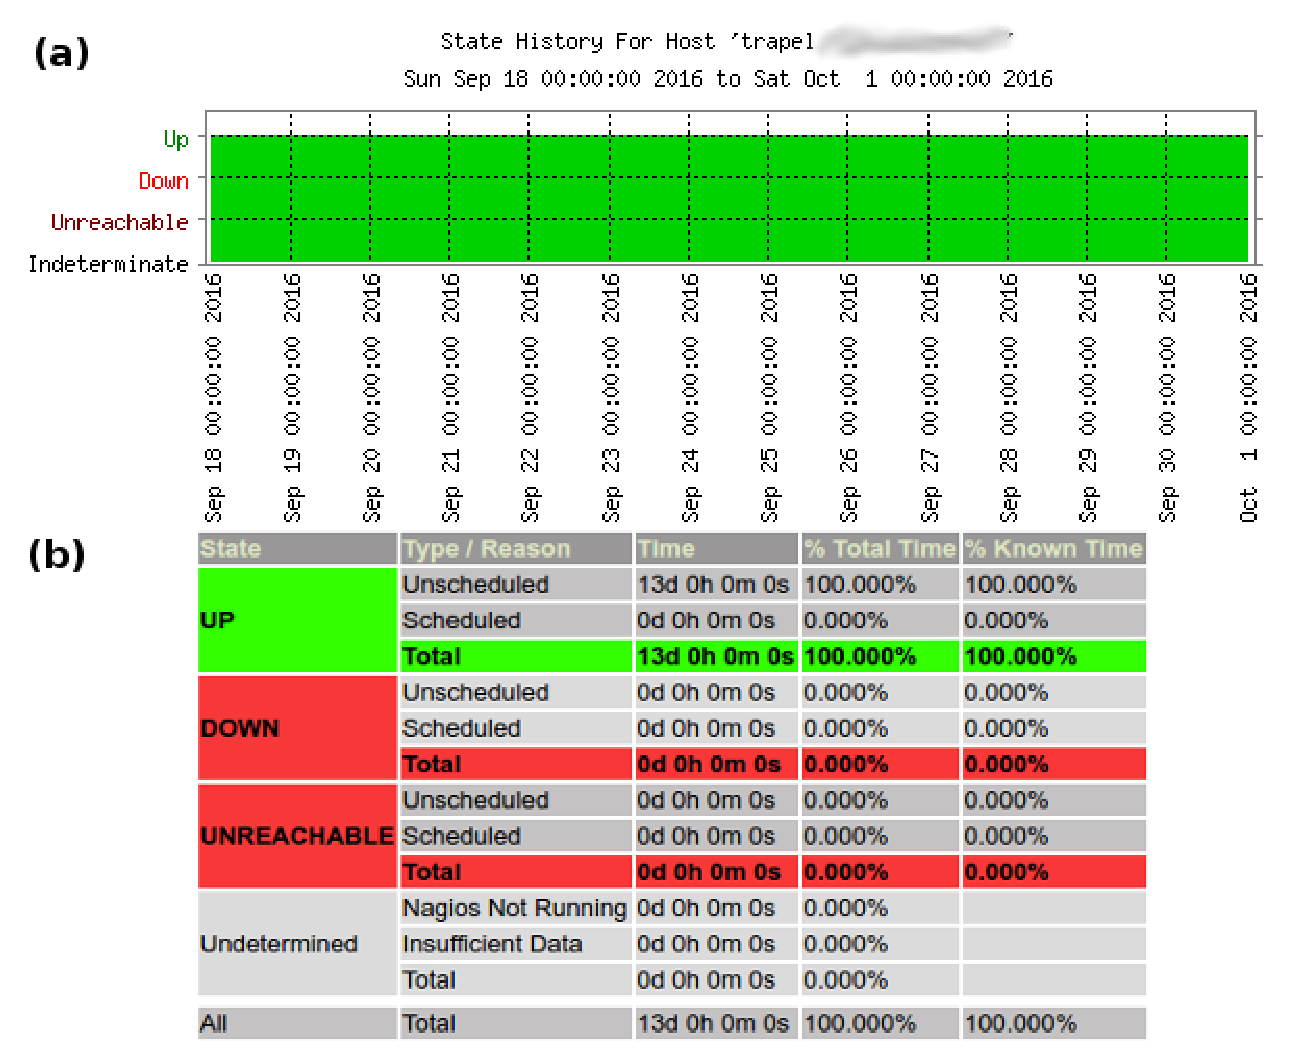
\includegraphics[width=350px]{img/teste2_trapel1.eps}
 \caption{Disponibilidade da máquina virtual, com o gráfico da disponibilidade (a) e a tabela com detalhes de tempo e percentual (b).}
 \label{fig:teste2_trapel1}
\end{figure}

Comparando os resultados da máquina virtual (Figura \ref{fig:teste2_trapel1} (b)) com os resultados dos nós 1 e 2 (Figura \ref{fig:teste2_brina1} 
(b) e Figura \ref{fig:teste2_piova1} (b)), pode-se perceber a diferença do \textit{uptime}, que fica entre 99,975\% e 99,976\% para os nós e 
100\% para a máquina virtual. Já nos gráficos da Figura \ref{fig:teste2_brina1} (a) e da Figura \ref{fig:teste2_piova1} (a), pode-se observar 
as duas reinicializações feitas.
\begin{figure}[h!]
 \centering
 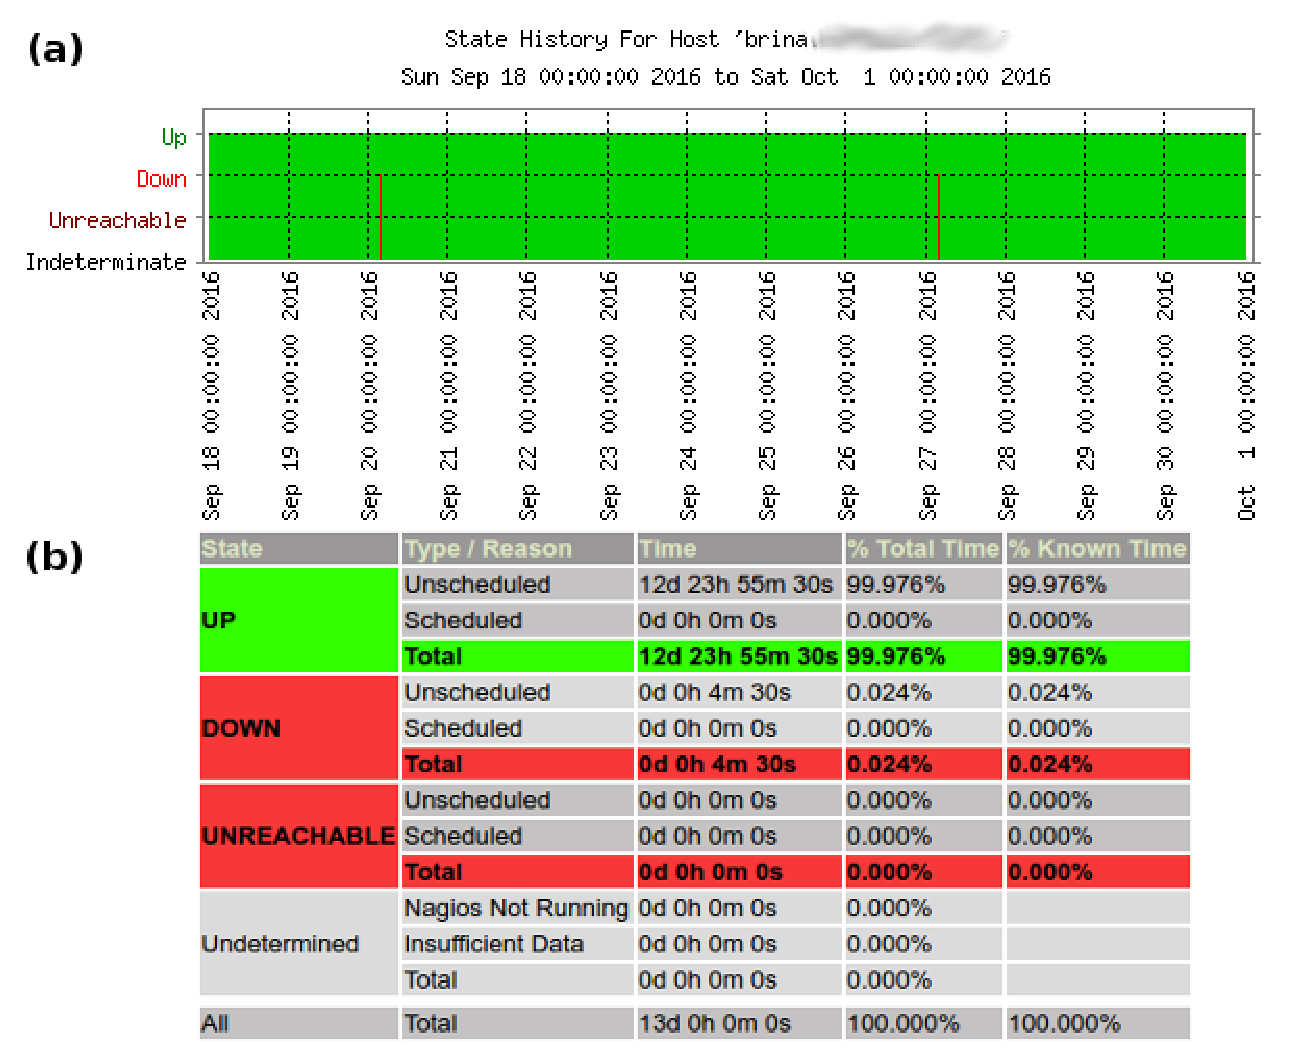
\includegraphics[width=350px]{img/teste2_brina1.eps}
 \caption{Disponibilidade do Nó 1, com o gráfico da disponibilidade (a) e a tabela com detalhes de tempo e percentual (b).}
 \label{fig:teste2_brina1}
\end{figure}

\begin{figure}[h!]
 \centering
 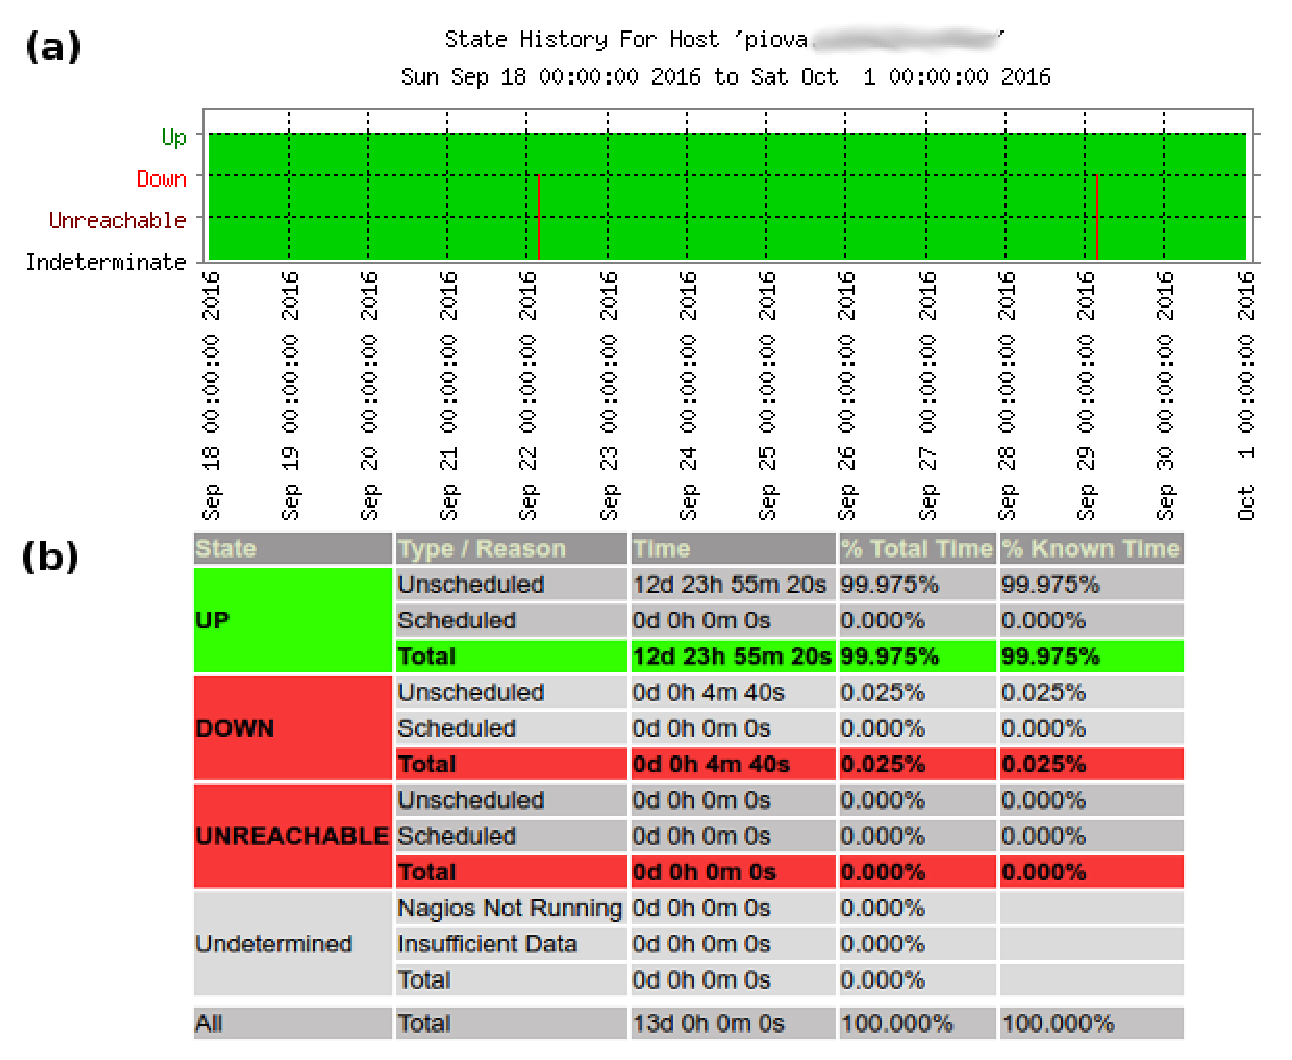
\includegraphics[width=350px]{img/teste2_piova1.eps}
 \caption{Disponibilidade do Nó 2, com o gráfico da disponibilidade (a) e a tabela com detalhes de tempo e percentual (b).}
 \label{fig:teste2_piova1}
\end{figure}

%log do pacemaker
%O processo de \textit{standby} feito pelo \textit{Pacemaker} está detalhado no \textit{log} abaixo:


\subsection{Teste 3 - Desligamento por software}
%Desligamento por software (reboot manual): 4 vezes para medir tempo de downtime dos servicos e dos nodes (servico nao critico)
%simulação de falha de software ou manutenção emergencial

Esse teste simula falhas de \textit{software} nos nós do \textit{cluster}, como por exemplo do \textit{software} de virtualização. Esse tipo de 
situação também pode ser necessário em uma manutenção emergencial, onde, por exemplo, é preciso desligar o servidor.

O procedimento deste teste é o seguinte:
\begin{itemize}
 \item Acessar o terminal do servidor de monitoramento;
 \item Executar comando \textit{ping} e medir o tempo de indisponibilidade (\textit{script} no Apêndice \ref{ap:scriptindisp});
 \item Acessar o terminal do nó que será reiniciado;
 \item Executar o comando \textit{reboot};
 \item Aguardar máquinas virtuais inicirem no outro nó e aguardar retorno do nó reiniciado;
 \item Finalizar a medição do tempo e \textit{ping}.
\end{itemize}

O procedimento deste teste foi executado 4 vezes no total, sendo que foram executadas 2 vezes em cada nó. A Tabela \ref{tab:teste3resultados}
demonstra os dados do servidor físico e do virtual.
% feito em 09/09

\begin{table}[h!]
\caption{Resultados do teste 3.}
\label{tab:teste3resultados}
\begin{center}
\begin{tabular}{|l|p{2.2cm}|p{2.5cm}|p{2.5cm}|p{1.5cm}|p{3cm}|}\hline
\textbf{Tipo} & \textbf{Média do tempo do teste} & \textbf{Média dos pacotes transmitidos} & \textbf{Média do percentual de pacotes perdidos} & \textbf{Latência média} & \textbf{Média do tempo de indisponibilidade} \\\hline
Servidores físicos & 260,53 segundos & 261 & 60,75 & 14,98 ms & 152,75 segundos \\\hline
Servidor virtual & 156,98 segundos & 158 & 18,75 & 0,222 ms & 5 segundos \\\hline
\end{tabular}
\end{center}
\end{table}

Pode-se observar que o tempo de indisponibilidade do servidor virtual é consideravelmente menor que o tempo do servidor físico, ele representa 
apenas 3,27\% do tempo de indisponibilidade do servidor físico. Além disso, pode-se perceber que o percentual de perda de pacotes é menor.
Este teste pode ser comparado com um caso que ocorreu a alguns meses na empresa, um servidor de virtualização, que é atualizado de forma automática,
foi reiniciado, porém ocorreu um erro na atualização e o servidor não pôde iniciar corretamente. Os serviços executados nele ficaram 
aproximadamente 6 horas indisponíveis.

\subsection{Comparação final da disponibilidade}
\label{section:comparacaofinal}
%Medição da disponibilidade dos serviços críticos por 1 mes (outubro) e comparar ao mês de setembro no ambiente antigo com 
%uma Reinicialização dos servidores físicos (reiniciados em 06/09/16)

Como já mencionado anteriormente, esta seção analisará os serviços críticos no ambiente final de produção que possui as máquinas virtuais
definidas na Seção \ref{section:maqservcrit}. 
%...foi mensurado a disponibilidade

... ??

adicionar gráficos de disponibilidade final dos serviços críticos:

%Medição através do comando ping e do Nagios, que utiliza ping para calcular o tempo de downtime
%Tabela com perda de pacotes, latencia, tempo de indisponibilidade X node fisico e maquina virtual


\section{Considerações finais}
